\documentclass[11pt]{book}
\usepackage [utf8] {inputenc}
\usepackage [T2A] {fontenc}
\usepackage[english, russian]{babel}

\usepackage{amssymb, amsthm, amsfonts}
\usepackage{amsmath}
\usepackage{mathtools}
\usepackage{needspace}
\usepackage{enumitem}

% разметка страницы и колонтитул
% \usepackage[left=1.5cm,right=2cm,top=1.5cm,bottom=1.1cm,bindingoffset=0cm]{geometry}
\usepackage{geometry}
 \geometry{
 a5paper,
%  total={148mm,210mm},
 left=10mm,
 top=15mm,
 right=10mm,
 bottom=10mm,
 }

\usepackage{fancybox,fancyhdr}
\fancyhf{}
\fancyhead[R]{\thepage}
\fancyhead[L]{\rightmark}
\fancyfoot{}
\fancyhfoffset{0pt}
\addtolength{\headheight}{13pt}
\pagestyle{fancy}


% Отступы
\setlength{\parindent}{0ex}
\setlength{\parskip}{3mm}

\usepackage{graphicx}
\usepackage{hyperref}

\usepackage{import}
\usepackage{xifthen}
\usepackage{pdfpages}

\newcommand{\incfig}[1]{%
    \def\svgwidth{\columnwidth}
    \import{./figures/}{#1.pdf_tex}
}

\usepackage{xcolor}
\definecolor{Aquamarine}{cmyk}{50, 0, 17, 100}
\definecolor{ForestGreen}{cmyk}{76, 0, 76, 45}
\definecolor{CarnationPink}{cmyk}{0, 0.349, 0.2118, 0}
\definecolor{Pink}{cmyk}{0, 100, 0, 0}
\definecolor{Cyan}{cmyk}{56, 0, 0, 100}
\definecolor{Gray}{gray}{0.3}

 % Цвета для гиперссылок
\definecolor{linkcolor}{HTML}{3f888f} % цвет ссылок
\definecolor{urlcolor}{HTML}{af0000} % цвет гиперссылок
 
\hypersetup{pdfstartview=FitH,
	linkcolor=linkcolor,urlcolor=urlcolor, colorlinks=true}

\theoremstyle{definition}
\newtheorem*{definition}{\underline{{\bf def}}}

\theoremstyle{theorem}
\newtheorem*{theorem}{\underline{{\bf thm}}}

\newtheorem*{st}{Утверждение}
\newtheorem*{prop}{Свойства}

\theoremstyle{plain}
\newtheorem*{name}{Обозначение}

\theoremstyle{remark}
\newtheorem*{rem}{Ремарка}
\newtheorem*{com}{Комментарий}
\newtheorem*{note}{Замечание}
\newtheorem*{prac}{Упражнение}
\newtheorem*{probl}{Задача}


\renewcommand{\o}{o}
\renewcommand{\O}{\mathcal{O}}

\renewcommand{\le}{\leqslant}
\renewcommand{\ge}{\geqslant}

\newcommand{\N}{\mathcal{N}}
\newcommand{\R}{\mathbb{R}}
\newcommand{\E}{\mathbb{E}}
\newcommand{\D}{\mathbb{D}}
\renewcommand{\P}{\mathcal{P}}
\newcommand{\PP}{\mathfrak{P}}
\newcommand{\cov}{\operatorname{cov}}
\newcommand{\MSE}{\operatorname{MSE}}

\def\selectedFont#1{\textsf{#1}}


\title{Дебильник}
\date{\today}
\author{Вячеслав Тамарин}

\begin{document}
\chapter{Дебильник}
\section{Многомерное нормальное распределение}
\begin{definition}
	\selectedFont{Стандартный гауссовский вектор} --- случайный $n$-мерный вектор $ Z = (Z_1, Z_2, \ldots Z_{n})$, координаты которого независимы и имеют распределение $ \N(0, 1)$.
\end{definition}

\begin{definition}[]
	\selectedFont{Гауссовский вектор} (\selectedFont{Нормальный вектор}) --- вектор, для которого существует матрица $ {\bf A} \in \R^{n \times m} $, стандартный гауссовский вектор $ Z \in \R^{m}$, и вектор $ b \in \R^{n}$ такие, что $ X = {\bf A}Z + b $.
\end{definition}

\begin{definition}[]
	\selectedFont{Распределение нормального вектора} $ X \in \R^{n}$ --- $ \N(\mu, {\bf \Sigma}) $ или $ \N_n(\mu, {\bf \Sigma}) $, где $ \mu = \E X$ и $ {\bf \Sigma} = \cov(X) $.
\end{definition}

\begin{definition}[]
	\selectedFont{Распределение хи-квадрат} с $ n$ степенями свободы --- распределение $ \chi^2(n) $ величины $ \chi^2 = Z_1^2 + Z_2^2 + \ldots + Z_{n}^2 $, где $ Z_{1}, Z_2, \ldots Z_{n}$ --- независимы $ \N(0, 1)$ величины. 
\end{definition}

\begin{definition}[]
	\selectedFont{Распределение Стьюдента} с $n$ степенями свободы --- распределение $T(n)$ величины $\frac{\sqrt{n}X}{\sqrt{Y}}$, где $X \sim \N(0, 1)$, $Y \sim \chi^2(n)$ и независимы.
\end{definition}

\begin{definition}[]
	\selectedFont{Распределение Фишера} со степенями свободы $n$ и $m$ --- распределение $F(n, m)$ величины $\frac{X / n}{Y / m}$, где $X \sim \chi^2(n)$, $Y \sim \chi^2(m)$ и независимы.
\end{definition}

\section{Условное матожидание}
\begin{definition}[]
	\selectedFont{Условное матожидание} $\E (Y \mid X)$ случайной величины $Y$ при условии случайной величины $X$ --- такая измеримая функция $g_0$ величины $X$, при которой $\E(Y - g(X))^2$ минимально для всех измеримых функций $g$.
\end{definition}
Условное матожидание --- ортогональная проекция $Y$ на линейное пространство всех измеримых функций $X$. То есть УМО --- единственная измеримая функция, которая удовлетворяет условию ортогональности:
 \[
\forall g \colon\E(Y - \E(Y \mid X)) g(X) = 0
.\] 

\section{Статистическая модель, выборка}
\begin{definition}[]
	\selectedFont{Статистическая модель} --- множество распределений $\PP$, которое, по нашему мнению, адекватно приближает $\P_D$. 
\end{definition}
\begin{definition}[]
	\selectedFont{Данные} $d$ --- реализация случайного элемента $D$, имеющего распределение $\P_D$.
\end{definition}
Статистические модели делят на:
\begin{itemize}
	\item \selectedFont{параметрические}, если $\PP = \{\P_0 \mid \theta \in \Theta \subset \R^{k}\}$.

		Пример: $\PP = \{\N(\mu, \sigma^2) \mid \mu \in \R, \sigma^2 \ge 0\}$.
	\item \selectedFont{непараметрические}, если $\PP = \{\P_0 \mid \theta \in  \Theta \subset V\}$, где $V$ не обязательно конечномерное.

		Пример: $\PP = \{\P^{\otimes n} \mid \int_{\mathfrak{X}}^{} x \P(dx) = 0 \}$
	\item \selectedFont{семипараметрические}, если $\PP = \{\P_0 \mid \theta \in \Theta \subset \R^{k} \times V\}$.

		Пример: линейная регрессия $Y = X \beta + \varepsilon$, $\beta \in \R^{k}$, $\E \varepsilon = 0$, $\D \varepsilon = \sigma^2$.
\end{itemize}
Если $D = [X_1, \ldots X_n]$ и $X_i$ независимы и имеют одинаковое распределение $\P_{X}$, $D$ называется \selectedFont{выборкой объема} $n$ и обозначается $X_{[n]}$, $\P_{X}$ --- генеральная совокупность.
В этом случае модель приобретает вид
$ \PP = \{\P^{\otimes n} \mid \P \in \PP_X\} $, где $\PP_X$ --- модель для $\P_X$.

\section{Формула Байеса, априорное, апостериорное распределение}
\begin{itemize}
	\item \selectedFont{Априорное распределение} --- наше ощущение относительно значения параметра до проведения эксперимента.
	\item \selectedFont{Апостериорное распределение} --- ощущение после получения данных эксперимента.
\end{itemize}
\begin{definition}[Формула Байеса]
	Здесь $p$ --- вероятность, $d$ --- данные, $\theta$ --- параметры.
	\[
	p(\theta \mid d) = \frac{p(d \mid \theta) \cdot p(\theta)}{p(d)}
	.\] 
	\begin{itemize}
		\item $p(\theta \mid d)$ --- апостериорное распределение,
		\item $p(d \mid \theta)$ --- правдоподобие,
		\item $p(\theta)$ --- априорное распределение,
		\item $p(d)$ --- вероятность данных.
	\end{itemize}
\end{definition}

\section{Расстояние Кульбака-Лейблера, энтропия}
Пусть мы принимаем случайные символы $x_1, \ldots x_{k}$, вероятность появления $x_{i}$ равна $p_i$, записываем с помощью битовой строки длины $l_i$. Тогда средняя длина символа равна 
\[
l = \sum_{i=1}^{k} p_i \cdot l_i
.\] 
Чтобы минимизировать $l$, необходимо подобрать следующие $l_i = - \log_2{p_i}$. И тогда средняя длина будет равна $H(x) \coloneqq - \sum_{i=1}^{k} p_i \cdot  \log_2{p_i}$, эта величина называется \selectedFont{двоичной энтропией сообщения}. Аналогично можно брать любой другой логарифм, мы будем использовать натуральный.

Для непрерывной величины можно завести \selectedFont{дифференциальную энтропию}:
\[
H(X) = - \int_{}^{} p(x) \log{p(x)} dx 
.\] 
Пусть случайная величина $X$ имеет функцию вероятности $p$, но мы кодируем символы, как-будто она имеет функцию вероятности $q$. Тогда средняя длина сообщения будет равна $- \sum_{i=1}^{k} p_i \cdot \log{q_i}$, эта величина называется \selectedFont{кросс-энтропией} $H(p \mid q)$ распределений $p$ и $q$.

$H(p \mid q)$ всегда будет больше $H(p)$, так как $H(p)$ минимально.
\begin{definition}[]
	Величина потери информации из-за использования $q$ вместо $p$ называется \selectedFont{расстоянием Кульбака-Лейблера} между $p$ и $q$:
	\[
	D_{KL} (p, q) = H(p \mid q) - H(p) = - \sum_{i=1}^{k} p_i \cdot \log{\frac{q_i}{p_i}}
	.\] 
\end{definition}
Для непрерывных величин все обобщается следующим образом 
\[
D_{KL} = - \int p_i \cdot \log{\frac{q_{i}}{p_i}}
.\] 

\section{Статистика...}
\subsection{Статистика}
Параметр или характеристика распределения --- функционал от этого распределения.
\begin{definition}[]
	\selectedFont{Статистика} ---  функция $\theta^*$ от данных $d$.
\end{definition}

Пусть модель $\PP_{[n]} = \{\P ^{\otimes n} \mid \P \in \PP\}$, искомая характеристика $\theta\colon \PP \to \R^{k}$.

\subsection{Несмещенность}
Чему равна оценка как случайная величина в среднем, если она равна характеристике?

\begin{definition}[]
	Оценка $\Theta^*$ называется
	\begin{itemize}
		\item \selectedFont{несмещенной}, если $\forall \P \in \PP\colon \E \theta^*(X_{[n]}) = \theta(\P)$, где $X_{[n]} \sim \P^{\otimes n}$,
		\item \selectedFont{асимптотически несмещенной}, если $\forall \P \in \PP\colon \E \theta^*(X_{[n]}) \to \theta(\P)$.
	\end{itemize}

	\selectedFont{Смещение} --- величина $b(\theta^*) = \E(\theta^*(X_{[n]})) - \theta(\P)$.

	\selectedFont{Среднеквадратичная ошибка} --- величина $\MSE(\theta^*) = \E \left( \theta^*(X_{[n]}) - \theta(\P) \right) ^2$.
\end{definition}
В общем случае 
\[
\MSE(\theta^*) = \D \theta^*(X_{[n]} + b^2(\theta^*)
.\] 
\begin{itemize}
	\item Выборочное среднее как оценка матожидания --- несмещенная оценка,
	\item Выборочная дисперсия как оценка дисперсии --- асимптотически несмещенная,
	\item Исправленная выборочная дисперсия как оценка дисперсии --- несмещенная оценка.
\end{itemize}

\subsection{Состоятельность}
\begin{definition}[]
	Оценка $\theta^*$ называется
	\begin{itemize}
		\item \selectedFont{состоятельной}, если $\forall \P \in \PP\colon \theta^*(X_{[n]}) \xrightarrow{\mathbb{P}} \theta(\P)$, где $X_{[n]} \sim \P^{\otimes n}$,
		\item \selectedFont{сильно состоятельной}, если $\theta^*(X_{[n]}) \xrightarrow{\text{п. н.}} \theta(\P)$.
	\end{itemize}
\end{definition}

\subsection{Асимптотическая нормальность}
\begin{definition}[]
	Оценка $\theta^*$ называется \selectedFont{асимптотически нормальной} с коэффициентом рассеивания (или просто дисперсией) $\sigma^2\bigl(\theta(\P)\bigr > 0$, если 
		\[
		\sqrt{n} \left( \theta^*(X_{[n]}) - \theta(\P) \right) \xrightarrow{d} \eta \sim \N(0, \sigma^2(\theta^*(\P)))
		.\] 
	В многомерном случае рассматривается ковариационная матрица вместо дисперсии.
\end{definition}
\begin{itemize}
	\item Выборочная дисперсия и второй момент --- асимптотически нормальная оценка.
	\item Из асимптотической нормальности следует состоятельность.
\end{itemize}

\subsection{Эффективность}
Рассмотрим класс оценок $K = \{\hat{\theta}\}$ параметра $\theta$.
\begin{definition}[]
	Оценка $\theta^* \in K$ называется \selectedFont{эффективной в классе} $K$, если \it{для любой другой оценки} $\hat{\theta} \in  K$ и \it{для любого исследуемого параметра} $\theta \in \Theta$ выполняется
	\[
	\MSE_{\theta}(\theta^*) \le \MSE_{\theta}(\hat{\theta})
	.\] 
\end{definition}
Класс несмещенных оценок
 \[
K_0 = \{\hat{\theta} \mid \E {\hat{\theta}} = \theta, \forall \theta \in \Theta\}
.\] 
\begin{definition}[]
		\selectedFont{Эффективная оценка} $\theta^*$, если эффективна в классе $K_0$.
\end{definition}
\begin{definition}[]
		\selectedFont{Асимптотически эффективной в классе} $K$, если для любой оценки $\hat{\theta} \in K$ и для любого $\theta \in  \Theta$ выполняется
			\[
			\overline{\lim_{n \to \infty}} \frac{\MSE(\theta^*)}{\MSE(\hat{\theta}}
			.\] 
\end{definition}

\subsection{Робастность}
\begin{definition}[]
	\selectedFont{Робастность} --- свойство оценки быть устойчивой к хвостам распределения.
\end{definition}
	Пусть $F$ --- распределение,  $\{G_{n}\}$ --- последовательность распределений, что
	\[
	\lvert F - G_{n}\rvert \coloneqq \underset{x}{\sup} \lvert F(x) - G_n(x) \rvert \to 0
	.\] 
\begin{definition}[]
	Характеристика $\theta$ обладает \selectedFont{качественной робастностью}, если $\theta(G_{n}) \to \theta(F)$
\end{definition}
Пусть также $\delta_x$ --- вырожденное распределение в точке $x$.
\begin{definition}[]
	\selectedFont{Загрязненное распределение} --- смесь $F_{x, \varepsilon} = (1-\varepsilon) F + \varepsilon \delta_x$.	
\end{definition}
\begin{definition}[]
	\selectedFont{Функция влияния} характеристики $\theta$ --- величина $$IF(x) = \lim_{\varepsilon \to 0+} \frac{\theta(F_{x, \varepsilon}) - \theta(F)}{\varepsilon}.$$
\end{definition}
\begin{definition}[]
	Характеристика $\theta$ называется \selectedFont{$B$-робастной} или \selectedFont{инфинитезимально робастной}, если $IF(x)$ ограничена.
\end{definition}
\begin{definition}[]
	\selectedFont{Асимптотическая толерантность} характеристики $\theta$ ---
	\[
	\tau = \inf \bigl\{ \varepsilon \mid \underset{x}{\sup}\lvert \theta(F_{x, \varepsilon} - \theta(F) \rvert = \infty \bigr\}	
	.\] 
\end{definition}

\subsection{Достаточность}
\begin{definition}[]
	Статистика $T(x) = \{T_1(x), \ldots , T_m(x))\}$ называется \selectedFont{достаточной}, если для всех 
	\begin{itemize}[noitemsep]
		\item $\theta \in \Theta$,
		\item $B \in \PP(\R^{n})$ и 
		\item $t = (t_1, \ldots , t_m)$
	\end{itemize}
	 условная вероятность $\mathbb{P}(X_{[n]} \in B \mid T(X_{[n]}) = t)$ не зависит от $\theta$.

	 То есть информация о $\theta$ в выборке полностью содержится в значении $T(x_{[n]})$.
\end{definition}
\begin{theorem}[факторизации]
	$T(x)$ достаточна, согда существуют функции $g$ и  $h$, что
	\[
	p(X_{[n]} = x_{[n]} \mid \theta) = g(T(x_{[n]}), \theta) h(x_{[n]})
	,\] 
	где $p$ --- вероятность или плотность.
\end{theorem}

\subsection{Полнота}
\begin{definition}[]
	Статистика $T$ называется \selectedFont{полной}, если для любой \it{измеримой} $g$ верно следствие
	\[
	 \forall \theta \in  \Theta\colon\E {g (T(X_{[n]}))} \equiv 0 \quad \implies \quad g(T(X_{[n]})) \overset{\text{п.н.}}{=} 0
	.\] 
\end{definition}


\section{Теоремы Колмогорова-Блэкуэлла-Рао и Лемана-Шеффе}
\begin{theorem}[Колмогорова-Блэкуэлла-Рао]
    Пусть $\theta^*$ --- оценка параметра $\theta$, $T$ --- достаточная статистика. Тогда \[
    \MSE(\theta^*) \ge \MSE(\E(\theta^* \mid T))
    .\] 
\end{theorem}
\begin{theorem}[Лемана-Шеффе]
    Пусть $\theta^*$ --- оценка параметра $\theta$, $T$ --- достаточная и полная статистика. Тогда $\E(\theta^* \mid T)$ --- единственная эффективная оценка в классе оценок со смещением $b(\theta^*)$.
\end{theorem}

\section{Доверительный интервал}
Пусть есть модель $\PP_{[n]} = \{\P^{\otimes n} \mid \P \in \PP\}$ и $\theta\colon \PP \to \R^{k}$ --- искомая характеристика.

\begin{definition}[]
	\selectedFont{Доверительный интервал} (точный доверительный интервал) с уровнем доверия $\gamma$ --- пара статистик $(\theta^*_L, \theta^*_R)$, такая что для любого $\P \in \PP$  и $X_{[n]} \sim \P^{\otimes n}$
	\[
	\mathbb{P} \left( \theta^*_L(X_{[n]}) \le \theta(\P) \le \theta^*_R(X_{[n]}) \right) = \gamma 
	.\] 

	Интервал называется
	\begin{itemize}
		\item \selectedFont{асимптотическим}, если
	\[
	\mathbb{P} \left( \theta^*_L(X_{[n]}) \le \theta(\P) \le \theta^*_R(X_{[n]}) \right) \xrightarrow{n \to \infty} \gamma 
	.\] 
		\item \selectedFont{центральным}, если
			\[
			\mathbb{P} \left( \theta^*_L(X_{[n]}) > \theta(\P) \right) = \mathbb{P} \left( \theta^*_R(X_{[n]}) < \theta(\P) \right) 
			.\] 
		\item \selectedFont{левым}, если
			\[
			\mathbb{P} \left( \theta^*_L(X_{[n]}) > \theta(\P) \right) = 0
			.\] 
		\item \selectedFont{правым}, если
			\[
			\mathbb{P} \left( \theta^*_R(X_{[n]}) < \theta(\P) \right) = 0
			.\] 
	\end{itemize}
\end{definition}

\section{Бутстреп}
\subsection{Параметрический бутстреп}
Если работаем с параметрической моделью, можем заменить $X=X(\theta)$ не на $X^*$, а на $X(\theta^*)$ и сэмплировать из этого распределения.
\subsection{Непараметрический бутстреп }
\paragraph{Рецепт}
\begin{enumerate}
	\item изготовим $N$ выборок $x^*_{[n], 1}, \ldots , x^*_{[n], N}$ из эмпирического распределения (рандом с возвращением)
	\item вычисляем $\theta^{b}_{i} = \theta^*(x^*_{[n], i}$, получаем бутстреповскую выборку $\theta^{b}_{[N]}$,
	\item по бутстреповской выборке оцениваем, что нужно.
\end{enumerate}
\paragraph{Ограничения}
\begin{itemize}
	\item $\theta^*$ --- plug-in оценка
    \item $\theta^*$ --- достаточно гладкая (обычно дифференцируема)
	\item у  $X$ достаточно много моментов (обычно конечная дисперсия)
	\item нужно генерировать большие выборки
	\item на очень больших данных трудозатратен
	\item на маленьких данных велика неустранимая ошибка
\end{itemize}

\section{Гипотеза, альтернатива...}
Пусть $\PP$ --- модель.
\subsection{Гипотеза и альтернатива}
\begin{definition}[]
	\selectedFont{Гипотеза} --- утверждение вида $H\colon \P_X \in  \PP_0 \subset \PP$.

	Если $\lvert \PP_0 \rvert = 1$, гипотеза называется \selectedFont{простой}, иначе \selectedFont{сложной}.

	\selectedFont{Нулевая гипотеза} --- гипотеза $H_0$, которую мы хотим проверить. Проверка гипотезы --- процесс принятия решения о том, противоречит ли она наблюдаемой выборке данных.

	\selectedFont{Альтернатива} --- гипотеза $H_1$, которая отражает, какие отклонения от нулевой гипотезы нам интересны.
\end{definition}
\subsection{Критерий}
\begin{definition}[]
	\selectedFont{Нерандомизированный критерий} (критерий) --- отображение $\varphi \colon d \to \{\text{принимаем}, \text{отвергаем}\} = \{H_0, H_1\} = \{0, 1\}$.
\end{definition}
Часто критерий устроен так: имеется
\vspace{-1.5em}
\begin{itemize}[noitemsep]
	\item \selectedFont{статистика критерия} $T$ и
	\item \selectedFont{критическое множество} $C$, и
\end{itemize}
\vspace{-1.5em}
\[
\varphi(d) = [T(d) \in C] = [d \in T^{-1}(C)]
.\] 
\begin{definition}[]
	\selectedFont{Рандомизированный критерий} --- отображение $\varphi\colon d \to [0, 1]$. Значение на данных $d$ определяется как реализация случайной величины $D(\varphi(d))$.
\end{definition}
Пусть мы согласны отвергать нулевую гипотезу пр условии, что она верна, но хотим делать это не очень часто. Пусть зафиксирован \selectedFont{уровень значимости}
\[
	\alpha\coloneqq \mathbb{P} (\varphi(D) = 1 \mid H_0) 
,\] 
который обычно является \textit{параметром критерия}, то есть, задавая его, мы определяем \textit{критическое множество} $C_{\alpha}$ такое, что
\[
	\mathbb{P} (T(D) \in C_{\alpha} \mid H_0) = \alpha
.\] 
Таким образом, для одного критерия определено семейство критических областей $\{C_{\alpha} \mid \alpha \in  [0, 1]\}$, где обычно $C_{\alpha} \subset C_{\alpha'}$, если $\alpha < \alpha'$.

\begin{definition}[]
	\selectedFont{Уровень значимости} --- параметр критерия, который регулирует, насколько часто мы будем отвергать нулевую гипотезу при условии, что она верна.
\end{definition}

\subsection{p-value}
Хотим оценить, насколько гипотеза противоречит наблюдаемым данным.
\begin{definition}[]
	\selectedFont{p-value} --- характеристика противоречия гипотезы наблюдаемым данным:
	\[
	\text{p-value} \coloneqq \arg \min \{\alpha \in [0, 1] \mid T(d) \in C_{\alpha}\}
	.\] 
	Другими словами, p-value --- минимальное значение уровня значимости для данного значения статистики критерия, при котором $H_0$ может быть отвергнута.

	Чем меньше p-value, тем больше гипотеза противоречит данным.
\end{definition}
\subsection{Ошибки разных родов}
\begin{definition}[]
	\selectedFont{Ошибка первого рода} --- событие $\varphi(D) = 1 \mid H_{0}$.
	Если уровень значимости совпадает с вероятностью ошибки первого роба, То критерий называется \selectedFont{точным}.
\end{definition}
Уровень значимости --- вероятность ошибки первого рода.

\begin{definition}[]
	\selectedFont{Ошибка второго рода} $\beta$ --- событие $\varphi(D) = 0 \mid H_{1}$, не отклонили нулевую гипотезу при условии, что была верна альтернатива.

	\selectedFont{Мощность} критерия --- вероятность $1 - \beta$ отклонить $H_0$ при условии, что верна $H_1$.
\end{definition}
Для заданного уровня значимости мы хотим иметь как можно более мощный критерий.
\subsection{Свойства критериев}
\begin{definition}[]
	\selectedFont{Несмещенность} --- мощность всегда не меньше ошибки первого рода, критерий не отдает предпочтение альтернативе. $1 - \beta \ge \alpha$ для всех простых гипотез из $\PP_0$ и простых альтернатив из $\PP_1$.
\end{definition}
\begin{definition}[]
	\selectedFont{Состоятельность} --- $\beta \xrightarrow{n \to \infty} 0$ для всех простых альтернатив из $\PP_1$.
\end{definition}
\begin{definition}[]
	\selectedFont{Асимптотичность} --- $\alpha \xrightarrow{n \to \infty}$ для всех простых гипотез из $\PP_0$.
\end{definition}
\begin{definition}[]
	\selectedFont{Наиболее мощный критерий} для данного уровня значимости $\alpha_0$ и простой альтернативы --- такой критерий $\varphi_1$, что для любого критерия $\varphi_2$ такого, что $\alpha(\varphi_2) \le \alpha_0$:
	\[
	\beta(\varphi_1) \le \beta(\varphi_2)
	.\] 
\end{definition}
\subsection{Размер эффекта}
Во многих случаях важна не только информация о p-value, но и величина наблюдаемого эффекта. Размеры эффекта бывают разные, использование того или иного размера эффекта зависит от контекста.

Вместо сравнения p-value с уровнем значимости для принятия статистического решения можно считать размер эффекта, сравнивать с минимальным практически интересным.

\section{Постановка гипотезы согласия. Критерии Колмогорова и Андерсона-Дарлинга}
\subsection{Постановка гипотезы согласия}
\begin{definition}[]
	\selectedFont{Гипотеза согласия} --- гипотеза о соответствии эмпирического распределения теоретическому распределению вероятностей. 
\end{definition}
Критерии для гипотез согласия бывают
\begin{itemize}
	\item общие --- применимые к любому предполагаемому распределению выборки,
	\item специальные --- применимые к гипотезам, формулирующие согласие с определенным свойством распределений;
\end{itemize}
\begin{itemize}
	\item для простых гипотез,
	\item для сложных гипотез.
\end{itemize}
\subsection{Критерий Колмогорова}
Сравнивает эмпирическое и истинное распределение. Для простой гипотезы.

Пусть $F_0$ непрерывна на $\R$. Определим статистику Колмогорова:
\[
	D_n(x_{[n]}) = \underset{x \in \R}{\sup} \lvert F_{n}^* - F_0(x) \rvert
.\] 
\begin{itemize}
	\item Если $H_0$ верна, то $D_n \left( X_[n] \right) \xrightarrow{\text{п.н.}} 0$;
	\item Если $H_0$ неверна, то $D_{n} \left( X_{[n]} \right) \xrightarrow{\text{п.н.}} \underset{x \in \R}{\sup} \lvert F_X(x) - F_0(x) \rvert > 0$.
\end{itemize}

\subsection{Критерий Андерсона-Дарлинга}
Для простой гипотезы.

Определим статистику критерия Андерсона-Дарлинга:
\begin{align*}
	A^2 &= n \int_{\R}^{} \frac{ \left( F_n^*(x) - F_0(x) \right) ^2}{F_0(x) \left( 1 - F_0(x) \right) } d F_0(x) = \\
		&= -n - \sum_{i=1}^{n} \frac{2i-1}{n} \left[ \ln F_0(X_{(i)} \mid \theta) + \ln \left( 1 - F_0(X_{(n+1-i)} \mid \theta \right)  \right] 
\end{align*}
Статистика $A^2$ при выполнении $H_0$ и непрерывности $F_0$ подчиняется табличному распределению. $C_{\alpha} = (a^2_{1-\alpha}, \infty)$.

\section{Постановка гипотезы о параметрах, проверка через доверительные интервалы, z-test, t-test, бутстреп из нулевой гипотезы}
\subsection{Постановка гипотезы о параметрах}
Пусть $\theta$ --- параметр ($X \sim F(x, \theta)$ ) или характеристика ($\theta = \varphi(F_x)$ ) распределения.

Нулевая гипотеза: $H_0 \colon \theta = \theta_0$.
Типичные альтернативы:
\begin{itemize}
	\item $H_1\colon \theta = \theta_1 \neq \theta_0$,
	\item $H_{>}\colon \theta > \theta_0$,
	\item $H_{<}\colon \theta < \theta_0$,
	\item $H_{\neq}\colon \theta \neq \theta_0$.
\end{itemize}

Усредненный рецепт:
\begin{enumerate}
	\item Выбираем оценку $\theta^*$ параметра $\theta$, распределение которой приближенно известно при данном $\theta$.
	\item В зависимости от альтернативы строим критическое множество:
		\begin{itemize}
			\item $H_1\colon \theta = \theta_1 > \theta_0$ или $H_{>}$, то $C_{\alpha} = (\theta^*_{1-\alpha}, \infty)$ \footnote{Здесь $\theta^*_{x}$ --- квантиль уровня $x$ распределения $\theta^* \mid H_0$} --- правое критическое множество;
			\item $H_1\colon \theta = \theta_1 < \theta_0$ или $H_{<}$, то $C_{\alpha} = (-\infty, \theta^*_{\alpha})$ --- левое критическое множество;
			\item $H_{\neq}$, то $C_{\alpha} = (-\infty, \theta^*_{\frac{\alpha}{2}} \cup (\theta^*_{1 - \frac{\alpha}{2}}, \infty)$ --- двустороннее критическое множество.
		\end{itemize}
	\item Если $\theta^* \in  C_{\alpha}$, то гипотезу можно отклонить, иначе --- нельзя.
\end{enumerate}

\subsection{Проверка через доверительные интервалы}
Усредненный рецепт:
\begin{enumerate}
	\item В зависимости от альтернативы строим доверительный интервал с уровнем доверия $\gamma = 1 - \alpha$:
		\begin{itemize}
			\item $H_1\colon \theta = \theta_1 > \theta_0$ или $H_{>}$, то $(\theta^*_{L}, \infty)$ --- правый доверительный интервал;
			\item $H_1\colon \theta = \theta_1 < \theta_0$ или $H_{<}$, то $(-\infty, \theta^*_{R})$ --- левый доверительный интервал;
			\item $H_{\neq}$, то $(\theta^*_{L} , \theta^*_{R})$ --- центральный доверительный интервал.
		\end{itemize}
\end{enumerate}

\subsection{z-test}
Пусть $X \sim \N(\mu, \sigma^2)$, $\mu$ неизвестно, $\sigma^2$ известно.

Если $H_0$ верна, то $Z = \frac{\sqrt{n} (\overline{X} - \mu_0)}{\sigma} \sim \N(0, 1)$ и $\overline{X} \sim N(\mu_0, \frac{\sigma^2}{n})$.

В зависимости от альтернативы подбираем критическую область:
\begin{table}[htpb]
	\centering
	\label{tab:crytical_space_z_test}

	\begin{tabular}{cccc}
		 & $\theta_1 > \theta_0$, $H_{>}$ & $\theta_1 < \theta_0$, $H_{<}$  & $H_{\neq}$ 
		\\
		\hline
		$C_{\alpha}$ & $(\mu_0 + z_{1-\alpha} \frac{\sigma}{\sqrt{n}}, \infty)$ &$(- \infty, \mu_0 + z_{\alpha} \frac{\sigma}{\sqrt{n}})$ & $\R \setminus (\mu_0 \pm z_{1-\frac{\alpha}{2}} \frac{\sigma}{\sqrt{n}})$
		\\
		\hline
		p-value & $1 - \Phi^{-1}(z)$ & $\Phi^{-1}(z)$ & $2(1-\Phi^{-1}(\lvert z \rvert))$
	\end{tabular}
	\caption{Критическая область для альтернативы}
\end{table}
\subsection{t-test}
Пусть $X \sim \N(\mu, \sigma^2)$, $\mu$ неизвестно, $\sigma^2$ неизвестно.

Если $H_0$ верна, то $T = \frac{\sqrt{n} (\overline{X} - \mu_0)}{s} \sim T(n-1)$.

В зависимости от альтернативы подбираем критическую область:
\begin{table}[htpb]
	\centering
	\label{tab:crytical_space_t_test}

	\begin{tabular}{cccc}
		 & $\theta_1 > \theta_0$, $H_{>}$ & $\theta_1 < \theta_0$, $H_{<}$  & $H_{\neq}$ 
		\\
		\hline
		$C_{\alpha}$ & $(\mu_0 + t_{1-\alpha} \frac{s}{\sqrt{n}}, \infty)$ &$(- \infty, \mu_0 + t_{\alpha} \frac{s}{\sqrt{n}})$ & $\R \setminus (\mu_0 \pm t_{1-\frac{\alpha}{2}} \frac{s}{\sqrt{n}})$
		\\
		\hline
		p-value & $1 - T^{-1}(t)$ & $T^{-1}(t)$ & $2(1-T^{-1}(\lvert t \rvert))$
	\end{tabular}
	\caption{Критическая область для альтернативы}
\end{table}

\subsection{Бутстреп из нулевой гипотезы}
Пусть мы хотим проверить гипотезу $H_0\colon \E X = \theta_0$.

Рецепт:
\begin{enumerate}
	\item Назначим каждому наблюдению $x_i$ в выборке вероятность $p_i$.
	\item Из пар $(x_i, p_i)$ изготовим дискретное распределение $F^*_p$.
	\item Подберем $p_i$ так, чтобы с одной стороны $\overline{x} = \theta_0$, а с другой $p_i$ максимизировали правдоподобие выборки $\mathcal{L}(p \mid x_{[n]}) = p_1 p_2 \ldots p_{n}$.
	\item Бутстрепим кучу выборок из получившегося $F_{p}^{*}$, считаем по ним выборочное среднее.
	\item Построим критическое множество в зависимости от альтернативы и проверим, лежит ли в нем выборочное среднее исходной выборки.
\end{enumerate}

\section{Постановка гипотезы однородности, ранговые критерии, permutation.}
\subsection{Гипотеза однородности}
Пусть $D = (x_1, x_2, \ldots , x_{n}, y_1, y_2, \ldots , y_{m})$ и
\begin{itemize}
	\item $\bf\sf X_{\text{\bf\sf нез}}$ --- $X_1, \ldots , X_{n}$ независимы и имеют одну функцию распределения $F(x)$,
	\item $\bf\sf Y_{\text{\bf\sf нез}}$ --- $Y_1, \ldots , Y_{n}$ независимы и имеют одну функцию распределения $G(x)$,
	\item $\bf\sf FG_{\text{\bf\sf c}}$ --- $F$ и $G$ непрерывны.
\end{itemize}
Гипотеза однородности: $H_0\colon F = G$.

Альтернативы:
\begin{itemize}
	\item неоднородности: $H_{ \neq }\colon \exists x ~ F(x) \neq G(x)$;
	\item доминирования $H_{ \ge }\colon \forall x ~F(x) \ge G(x) \wedge \exists x ~ F(x) > G(x)$;
	\item правого сдвига $H_{ \to }\colon \forall x ~F(x) = G(x + \theta) \wedge \theta > 0$;
	\item масштаба $H_{ \leftrightarrow }\colon \forall x ~F(x) = G(x \theta) \wedge 1 \neq \theta > 0$;
\end{itemize}
\subsection{Ранговые критерии}
\subsubsection{Критерий Уилкоксона ранговых сумм}
Используется для проверки гипотезы $H_0$ против $H_{ \ge }$ и $H_{ \to }$.

Идея: Если $H_0$ верна, то $Y_{(i)}$ распределены в вариационном ряду $Z$ равномерно.

Статистика критерия: $W = \sum_{i=1}^{m} R(Y_i)$.
\[
W \in \left[ \frac{m(m+1)}{2},  mn + \frac{m(m+1)}{2} \right] 
.\] 
\[
C_{\alpha} = \left( c_{\alpha}, mn+\frac{m(m+1)}{2}  \right)
.\] 
\subsubsection{Критерий Манна-Уитни}
Используется для проверки гипотезы $H_0$ против $H_{ \ge }$ и $H_{ \to }$.

Идея аналогичная.

Статистика критерия: $U = \sum_{i=1}^{n} \sum_{j=1}^{m} [x_i < y_j]$.

Нетрудно видеть, что $U = W - \frac{m(m+1)}{2}$, поэтому $U \in [0, mn]$.
\[
C_{\alpha} = (c_{\alpha}, mn)
.\] 

Ценность этих критериев в том, что можно проверять выборки из величин, сравнимых только качественно.

\subsubsection{Критерий знаковых рангов Уилкоксона}
Пусть 
\begin{itemize}
	\item $\bf\sf E_{\text{\bf\sf нез}}$ --- $E_1, \ldots , E_{n}$ независимы,
	\item $\bf\sf E_{\text{\bf\sf сим}}$ --- $E_1, \ldots , E_{n}$ распределены одинаково и симметричны относительно нуля.
\end{itemize}
Рассматриваем вариационный ряд величин $\lvert z_i \rvert$.

Статистика критерия: $T = \sum_{i=1}^{n} R(\lvert z_{i} \rvert) [z_i < 0]$.

Для маленьких $n$ квантили смотрим в таблице, для больших можем использовать Монте-Карло или аппроксимацию:
\[
	\frac{T - \frac{n(n+1)}{4}}{\sqrt{\frac{n(n+1)(2n+1)}{24}}} \to \eta \sim \N(0, 1)
.\] 
\subsection{Permutation}
Пусть выполнено $\bf\sf E_{\text{\bf\sf нез}}$ и $\bf\sf E_{\text{\bf\sf сим}}$. 
 \begin{enumerate}
	\item Случайно умножаем $z_i$ на $1$ и $-1$ ;
	\item Для полученного вектора считаем медиану;
	\item Повторяем так $N$ раз;
	\item Считаем, сколько медиан меньше $\operatorname{med}(z)$ и делим на  $N $.
\end{enumerate}

Пусть $y_{[n]}^{p}$ --- случайная перестановка $y_{[n]}$. Если верна $H_0$, то все выборки $(x, y^{p})_{[n]}$ <<равновероятны>>.
План-капкан:
\begin{enumerate}
	\item генерируем случайную перестановку $y^{p}$,
	\item вычисляем значение требуемой статистики $r(x, y^{p})$,
	\item повторяем $N$ раз,
	\item считаем, какая доля оказалась меньше, чем $r(x, y)$.
\end{enumerate}

Пусть есть статистика $\theta^*(x_{[n]}, y_{[m]})$. Мы можем представить ее в виде $\theta^* = \theta^*(z_v, u)$.

Пусть $u^{p}$ --- случайная перестановка $u$. Тогда, если верна $H_0$, то
\[
\mathbb{P} \left( \theta^*(z_v, u^{p}) < \theta^*(z_v, u) \right)  =
\frac{\# \{u^{p} \mid \theta^*(z_v, u^{p}) < \theta^*(z_v, u) \} }
{{{n+m} \choose{n}}}
.\] 
Статистика критерия:
\[
C(x_{[n]}, y_{[m]}) = 
\frac{\# \{u^{p} \mid \theta^*(z_v, u^{p}) < \theta^*(z_v, u) \} }
{{{n+m} \choose{n}}}
,\] 
\[
C_{\alpha} \in \left\{  (1- \alpha, 1), ~ (0, \alpha), ~ (0, \tfrac{\alpha}{2}) \cup (1 - \tfrac{\alpha}{2}, 1) \right\}
.\] 
{\bf Killer Feature}: ошибка первого рода в точности равна  $\alpha$.

\section{Дисперсионного анализ, корреляционного анализ, таблицы сопряженности.}
ANOVA --- ANalysis Of VAriance.
\subsection{Однофакторный дисперсионный анализ}
\begin{itemize}
	\item имеется несколько выборок $x^{1}_{[n_1]}, \ldots , x^{k}_{[n_k]}$,
	\item которые являются наблюдениями случайных величин
		\[
		X_{i, j} = \mu + \beta_j + \varepsilon_{i, j}, \quad i = 1, \ldots n, j = 1, \ldots k
		,\] 
		где $\mu$ --- общее среднее, $\beta_j$ --- систематическая ошибка (или эффект фактора) выборки $x^{j}_{[n_j]}$ и $\varepsilon_{i, j}$ --- случайная ошибка.
\end{itemize}
\subsubsection{Постановка задачи дисперсионного анализа}
Пусть $\mu_j = \mu + \beta_j$, $N = n_1 + \ldots + n_j$ и
\begin{itemize}
	\item $\bf\sf E_{\text{\bf\sf нез}} $ --- все ошибки $\varepsilon_{i, j}$ независимы,
	\item $\bf\sf E_{\text{\bf\sf с}} $ --- все ошибки $\varepsilon_{i, j}$ имеют одинаковое непрерывное распределение.
\end{itemize}
Гипотеза $H_0\colon \mu_1 = \mu_2 = \ldots = \mu_{k}$.

Альтернатива $H_1\colon \exists i, j\colon \mu_{i} \neq \mu_{j}$.

\subsubsection{Критерий Андерсона-Дарлинга для ANOVA}
Пусть выборки $X_{[n_i]}^{i}$ независимы и имеют распределение $F_i$.

Гипотеза $H_0\colon F_1 = F_2 = \ldots = F_{k}$.

Альтернатива $H_1\colon \exists i, j\colon F_i \neq F_j$.
\[
A^2_{k, N} = \sum_{i=1}^{k} n_i \int_{\R}^{} \frac{ \left( F_{n_i}^2(x) - H_N(x) \right) ^2}{H_{N}(x) \left( 1 - H_N(x) \right) } d H_N (x)
,\] 
где $H_{N} = \frac{1}{n} \sum_{i=1}^{k} n_i F_{n_i}^*$ --- эмпирическая функция распределения объединенной выборки $Z = \left( X_{[n_1]}, \ldots , X_{[n_k]} \right) $.

Если повторений нет, то можно переписать следующим образом:
\[
A_{k, N}^2 = \frac{1}{N} \sum_{j=1}^{k} \frac{1}{n_j} \sum_{i=1}^{N-1} \frac{(Nc_{i, j} - j n_j)^2}{i(N-i)}
,\] 
где $c_{i, j}$ --- количество наблюдений $X_{[n_j]}^{j}$ меньших  $Z_{(i)}$.

\subsection{Постановка задачи корреляционного анализа}
\paragraph{Гипотеза независимости}
Имеется выборка $(x, y)_{[n]}$ --- реализация $(X, Y)_{[n]}$, при этом $X_i$ имеет функцию распределения $F_{X}$, а $Y_i$ имеет $F_Y$.

Гипотеза $H_0\colon F_{X, Y}(x, y) = F_{X}(x) F_{Y}(y)$.

Предполагаем гипотезу независимости, но проверять будем отсутствие корреляции.

\subsection{Таблица сопряженности}
\begin{figure}
	\centering
    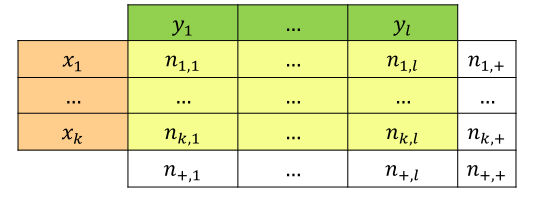
\includegraphics[scale=0.5]{./figures/table.png}
\end{figure}
Три схемы, в которых они возникают:
\begin{itemize}
	\item Гипотеза однородности: строка $i$ --- реализация случайной величины $x_i$ с вероятностями $\mathbb{P}(x_i = y_j) = q_{i, j}$, $\sum_{}^{} q_{i, j} = 1$ и с заданным числом наблюдений $n$ (то есть $ \forall i\colon n =  n_{i, +}$).
		\[
		H_{I}\colon q_{i, j} = q_{+, j}, \quad q_{+, j} = \frac{1}{k} \sum_{i}^{} q_{i, j}
		.\] 
		Пример: $k$ кубиков, каждый подбросили $n$ раз, $n_{i, j}$ --- количество выпадений числа $j$ у кубика $i$.
	\item Гипотеза независимости: вся таблица --- реализация случайной величины $\xi$ с 
		$\mathbb{P}\left(\xi = (x_i, y_j)\right) = p_{i, j}$,
		где $\sum_{i, j}^{} p_{i, j} = 1$, и с $n_{*, *}$ наблюдениями.
		\[
		H_{II}\colon \mathbb{P}\left(\xi = (x_i, y_j)\right) = \mathbb{P}(\xi_{x} = x_i) \mathbb{P}(\xi_{y} = y_j)
		.\] 
		Пример: выборка двумерной случайной величины $(x, y)_{[n]}$, для которой построена гистограмма с ячейками $\delta^{x}_i \times \delta^{y}_j$.
	\item Гипотеза мультипликативности: каждая ячейка --- реализация случайной величины.
		
		Важный частный случай: когда $n_{i, j}$ независимы и имеют распределение Пуассона с параметрами $\lambda_{i, j}$. Тогда их сумма тоже имеет распределение Пуассона.
		\[
		H_{III} \colon  \lambda_{i, j} = \frac{a_{i} b_{j}}{c}, \quad a_i = \sum_j \lambda_{i, j}, b_{j} = \sum_i \lambda_{i, j}, c = \sum_{i, j}^{} \lambda_{i, j}
		.\] 
		Пример: $n_{i, j}$ --- количество заболевших с диагнозом $i$ в районе $j$ за некоторый фиксированный промежуток времени.
\end{itemize}
Все три гипотезы проверяются с помощью критерия хи-квадрат.

Статистика критерия:  \[
\xi^2 = n_{+, +} \sum_{i, j}^{} \frac{\left( n_{i, j} - \frac{n_{i, +} n_{+, j}}{n_{+, +}}\right) ^2}{n_{i, +}n_{+, j}}
.\] 
Если гипотеза $H_{I}$, $H_{II}$ или $H_{III}$ верна, то
\[
\xi^2 \xrightarrow{d} \eta \sim \xi^2\left((k-1)(l-1)\right)
,\] 
\[
C_{\alpha} = (\xi^2_{1-\alpha}, \infty)
.\] 

\section{Линейная регрессия: постановка, теорема Гаусса-Маркова, базовые свойства, беды с регрессией.}
\subsection{Регрессионный анализ}
\begin{itemize}
	\item Данные: многомерная выборка $(X, Y)_{[n]}$, $X_i \in \R^{k}$, $Y_i \in \R$ и семейство функционалов $\{f(\cdot \mid \beta) \mid \beta \in B\}$.
	\item $Y \coloneqq Y_{[n]}$ --- зависимая переменная, target.
	\item $X \coloneqq X_{[n]}$ --- факторы, фичи.
\end{itemize}
Считаем, что $y_i \approx f(X_i, \beta_0)$, то есть $y_i = f(X_i, \beta_0) + \varepsilon_i$, где $\varepsilon_i$ --- шум, обладающий какими-то свойствами, например, $\E \varepsilon_i = 0$.

Хотим по $(X, Y)$ найти наилучшую в каком-то смысле оценку $\beta^*$ параметра $\beta_0$. Смысл задается функционалом качества $Q(\beta)$.

\subsection{Линейная регрессия}
\subsubsection{Модель:}
\begin{itemize}
	\item $D = (X, Y)$
	\item  $Y \in \R^{n}$, $Y = X \beta_0 + \varepsilon$,
	\item $X \in \R^{n \times k}$ фиксирована и известна, $\operatorname{rank} X = k$,
	\item  $\beta_0 \in \R^{k}$ фиксирован и неизвестен,
	\item $\varepsilon \in  \R^{n}$, $\E \varepsilon = 0$,
	\item $\D \varepsilon_i = \sigma^2$ --- \selectedFont{гомоскедастичность}б
	\item  $ \forall i \neq j\colon\cov(\varepsilon_i, \varepsilon_j) = 0$ --- некоррелированность.
		\[
		\cov (\varepsilon) = \sigma^2 I
		.\] 
\end{itemize}
Ищем оценку $\beta^*$ в виде $\arg \min_{\beta \in \R^{k}} \sum_{i=1}^{n} \left( y_i - X_{i, *} \beta \right) ^2$.
Она называется оценкой \selectedFont{метода наименьших квадратов} или \selectedFont{МНК-оценкой}.
\begin{theorem}[Гаусс-Марков]
	Если $X$ имеет ранг $k$, ошибки гомоскедастичны и некоррелированы, то
	\begin{itemize}
		\item $\beta^*$ --- несмещенная оценка $\beta_0$,
		\item $\cov(\beta^*) = \sigma^2(X^{\top} X)^{-1}$,
		\item $\beta^*$ --- эффективная оценка в классе несмещенный линейных оценок\footnote{Линейные оценки --- оценки вида $\beta = f(X) y$, оптимальность означает, что $ \forall c \in \R^{k} \colon c^{\top}\cov(\beta^*) c \le c^{\top} \cov( \beta^*) c$ }.
	\end{itemize}
\end{theorem}
\subsubsection{Базовые свойства}
\begin{itemize}
	\item $\frac{\beta^*_i-\beta_i}{s(\beta^*_i)} \to \N(0, 1)$, где $s^2(\beta^*_i = \hat{\sigma} \left( X^{\top} X \right)^{-1}_{i, i}$ и $\hat{\sigma}^2 = \frac{RSS}{(n-k)}$,
	\item $\hat{\sigma}^2$ является несмещенной и состоятельной оценкой $\sigma^2$. 
\end{itemize}

Дисперсия target --- сумма дисперсии предсказания и дисперсии ошибки:
\[
\D y_i = \D \left( f (X_i \mid \beta_0) + \varepsilon_i \right)  = \D \left( f(X_i \mid \beta_0) \right) + \D \varepsilon_i
.\] 
\begin{itemize}
	\item $TSS = \sum (Y_i - \overline{Y})^2 $ --- total sum of squares (типа $n \D y_i$),
	\item $ESS = \sum (Y_i^* - \overline{Y})^2 $ --- explained sum of squares (типа $n \D \left( f(X_i \mid \beta_0 \right)	$),
	\item $RSS = \sum (Y_i - Y_i^*)^2 $ --- residual sum of squares (типа $n \D \varepsilon_i$),
\end{itemize}
\[
TSS = ESS + RSS
.\] 
\subsubsection{Беды с регрессией}
\paragraph{Беды с предположениями}
\begin{itemize}
	\item Неверная спецификация модели: $Y$ не линейно выражаются через $X$. Смотрим на график остатков против предсказания. Надо чтобы было линейно. Можно переделать модель.
	\item Непостоянная дисперсия остатков: дисперсия (ковариация) зависит от $X_i$.
	\item Корреляция остатков: возникает, когда наблюдения близки во времени или пространстве.
\end{itemize}
\paragraph{Беды с данными}
\begin{itemize}
	\item Выбросы: $X_i$ типичный, а $Y_i$ нетипичный.
	\item Разбалансировка: $X$ большой и $Y$ большой.
	\item Мультиколлинеарность:  $k$ факторов, но $\operatorname{rank} X < k$, есть линейные зависимости или нестрогая $\operatorname{rank} X = k, \operatorname{cond} \gg 1$.
\end{itemize}

\end{document}
